\chapter{Background: Deep Program Induction} 
\label{ch:promise}

\section{The Quest of Automatic Programming}

\label{sec:quest}

\emph{Automatic programming} or \emph{program synthesis} is any technological setup wherein the task of writing computer programs is automated. 
First introduced in science fiction \cite{jenkinsLogicNamedJoe1946}, it is now an active area of technical research.
Program synthesis systems are defined by what type of task \emph{specification} they admit, whether and how the generated programs are verified, whether and how pre-existing programs are incorporated \cite{gulwaniDimensionsProgramSynthesis2010}, see figure \ref{fig:ap}.

\begin{figure}
    \centering
    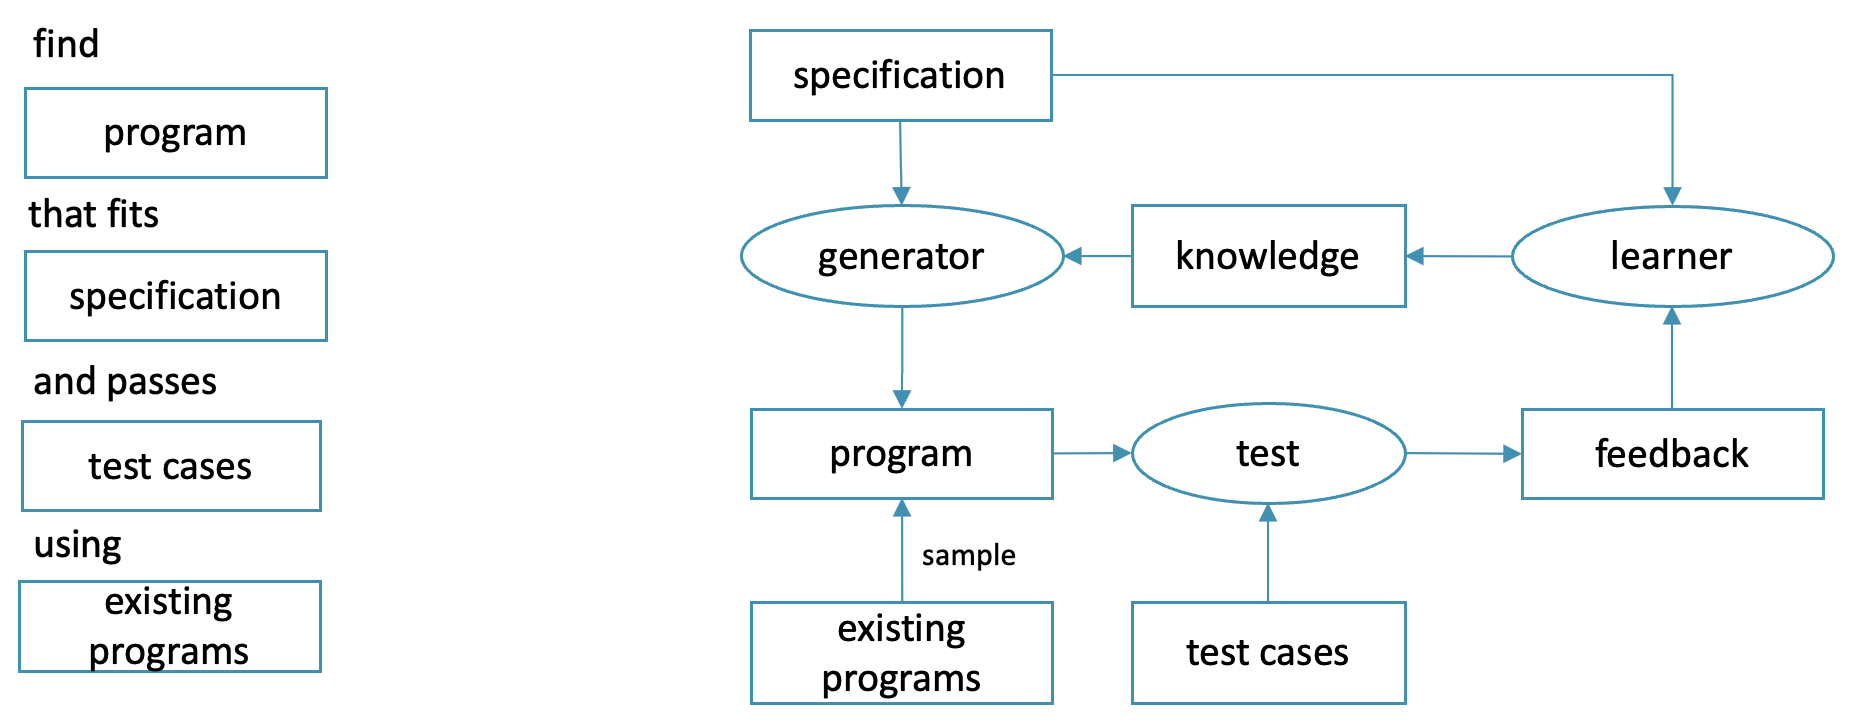
\includegraphics[width=\linewidth]{ap.png}
    \caption{Possible components of an automatic programming system}
    \label{fig:ap}
\end{figure}

This definition is purposefully broad and includes, for example, the compiler \cite{penjamDeductiveInductiveMethods2003,patrickmckenzie[@patio11]GlibLineHave2023}: a program synthesis system that turns a specification in the form of a program in a programming language designed for ease of use ("spec text" in figure \ref{fig:compiler}) into a program in a programming language designed for ease of deployment ("program" in figure \ref{fig:compiler}).

\begin{figure}
    \centering
    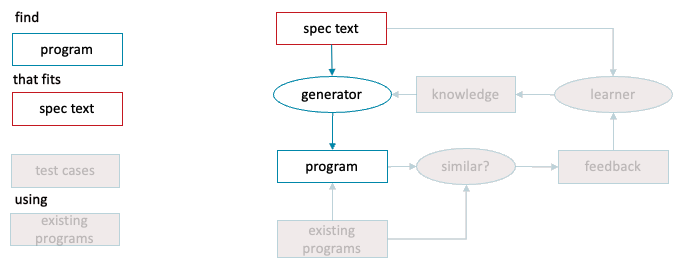
\includegraphics[width=\linewidth]{compiler.png}
    \caption{Compiler, schematic definition}
    \label{fig:compiler}
\end{figure}

The ambition of the field, however, extends far beyond compilers \cite{campbellAutomatedCodingQuest2020}.
The goal is to impose as few constraints as possible onto the \emph{specification} and ultimately automate the generation of programs for any free-form specification, such as a short textual \cite{zanLargeLanguageModels2023} prompt or a diagram \cite{koziolekLLMbasedControlCode2023}, even a hand-drawn sketch \cite{chatgptmodderChatgptCanNow2023}.

% TODO: examples for the above

\newpage
\section{Taxonomy of tasks}
\label{sec:ps-task-taxonomy}

\subsection{Code translation}

The humble compiler from section \ref{sec:quest} is an instance of \emph{code translation}: a \emph{program synthesis} setup where the specification is given as text (highlighted in figure \ref{fig:nl2ml}), either in a natural language (\emph{NL2Code translation} \cite{wangNaturalLanguageCode2023, zanLargeLanguageModels2023}) or in a programming language (\emph{code2code translation} \cite{radfordImprovingLanguageUnderstanding})
Code to natural language translation is studied as well \cite[section 5.1]{leDeepLearningSource2020}, but it is less common and out-of-scope for this work.
Intelligent conversational assistants (\href{https://chat.openai.com/}{ChatGPT}, \href{https://gemini.google.com}{Gemini}, \href{https://claude.ai/}{Claude}) with program synthesis functionality operate in the translation paradigm as they translate a text specification into code.

\begin{figure}
    \centering
    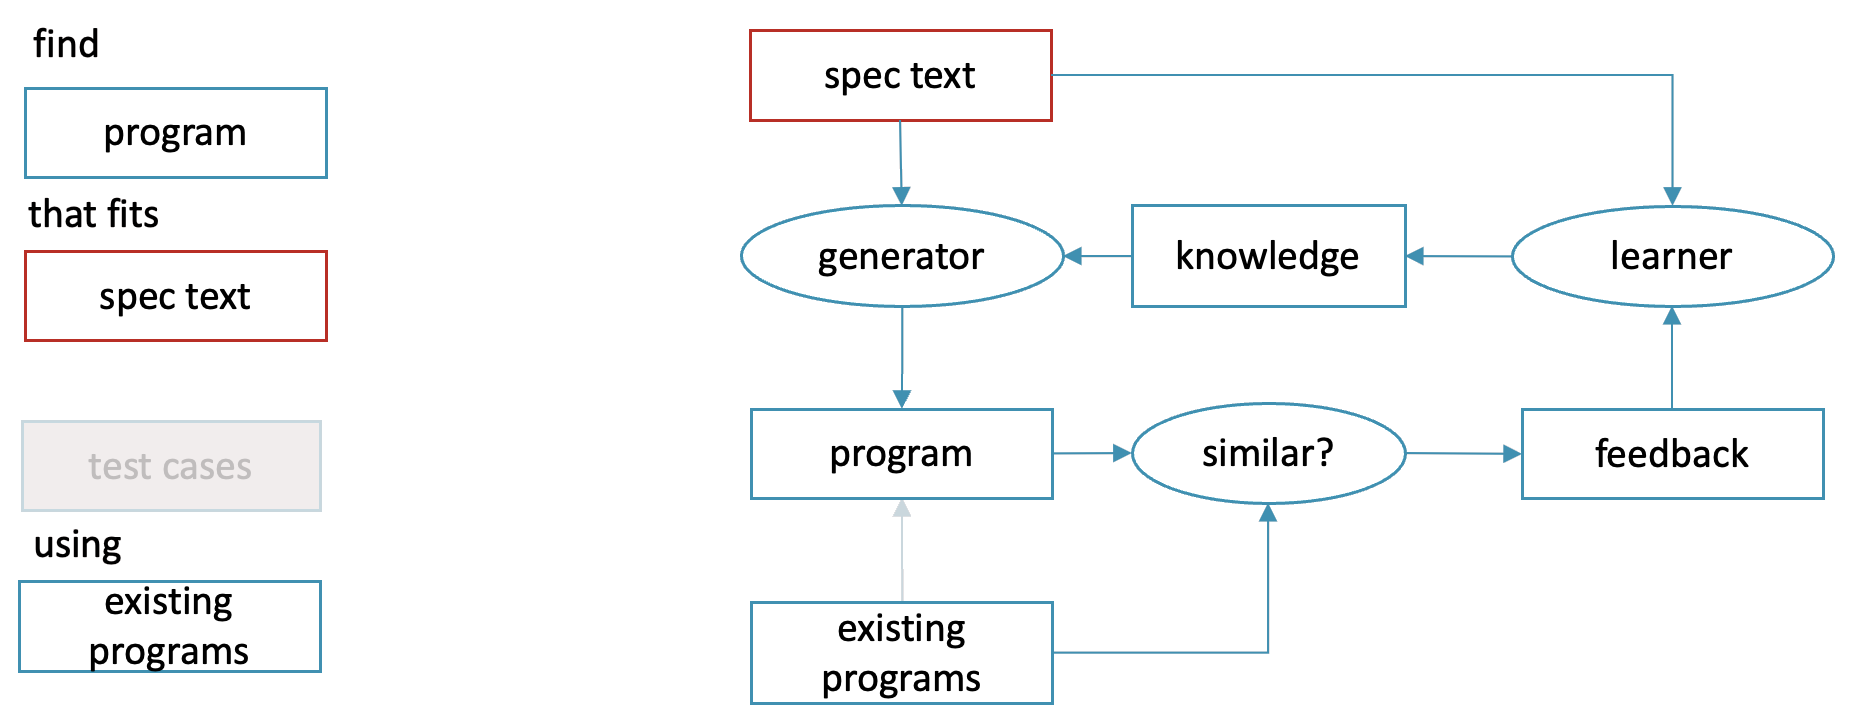
\includegraphics[width=\linewidth]{nl2ml.png}
    \caption{Code translation, schematic definition}
    \label{fig:nl2ml}
\end{figure}

\subsection{Programming by example}

Another approach to specification is specifying the expected output of the program. Or, since in most interesting programs the output depends on the input, \emph{input-output pairs} (highlighted in figure \ref{fig:pbe}). This task is known as \emph{programming by example} \cite{halbertProgrammingExample1984, psb2}.

\begin{figure}
    \centering
    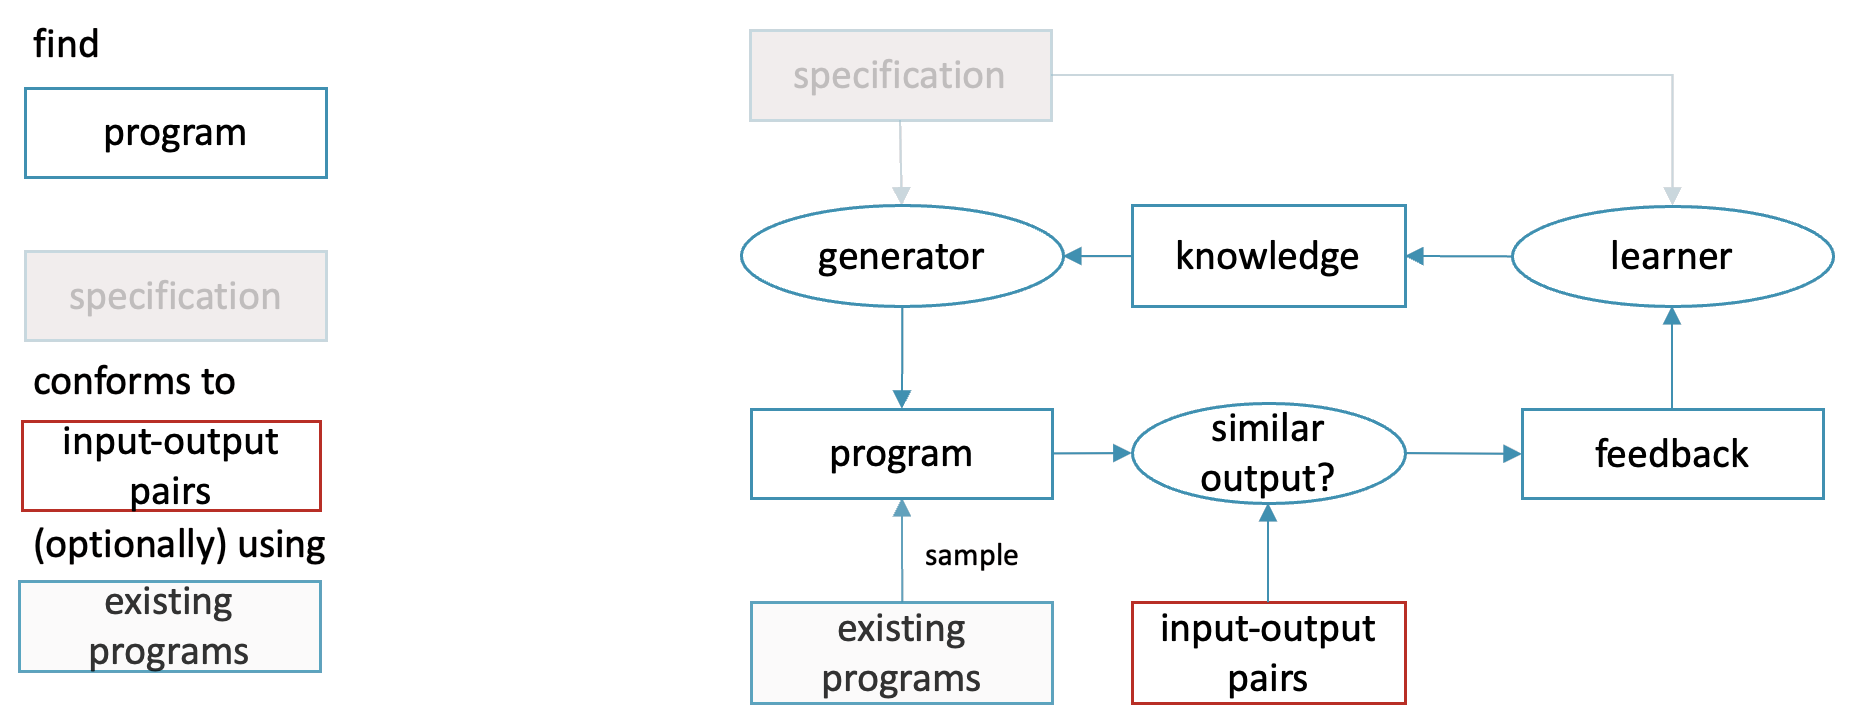
\includegraphics[width=\linewidth]{pbe.png}
    \caption{Programming by example, schematic definition}
    \label{fig:pbe}
\end{figure}

The goal of a programming by example system is to find a program $f$ such that $\mloutputvec=f(\mlinputvec)$ for a given vector of input-output pairs $(\mlinputvec,\mloutputvec)$. 
Note that this is exactly the definition of \emph{supervised learning}~\cite{cunninghamSupervisedLearning2008}.
Indeed, \emph{programming by example} is an unusual type of \emph{supervised learning}, one where the trained model is expressed as source code.

The prime application of \emph{programming by example} is \emph{data wrangling} tools such as Microsoft Excel \cite{gulwani2016:programming} where it is used as a data extrapolation tool: if a formula $f$ can be synthesized that satisfies $\mloutputvec=f(\mlinputvec)$, one can generate $\mloutputvec '=f(\mlinputvec ')$ for future values $\mlinputvec '$.
\emph{Programming by example} is also used in scientific domains to generate formulas that fit experimental observations, where it is known as \emph{symbolic regression} \cite{makkeInterpretableScientificDiscovery2022}.

\subsection{RLCEF}
\label{sec:rlcef}

Not every task, however, can be easily described with input-output examples. 
Take chess: it's relatively simple to evaluate the performance of a chess-playing program, but what are the \emph{correct} moves? 
That is simply not known in advance.
Given enough trial and error it's still possible to generate a correct program with such black box specification, a task known as \emph{Programmatically Interpretable Reinforcement Learning} \cite{pirl}, later renamed to Reinforcement Learning from Code Execution Feedback (RLCEF) \cite{douStepCoderImproveCode2024, gehringRLEFGroundingCode2025, liuRLTFReinforcementLearning2023, PoolsideAnnouncingOur, shojaeeExecutionbasedCodeGeneration2023, yangIntercodeStandardizingBenchmarking2023}.
The newer term will be preferred from now on\footnote{for search engine optimization reasons}.

\begin{figure}
    \centering
    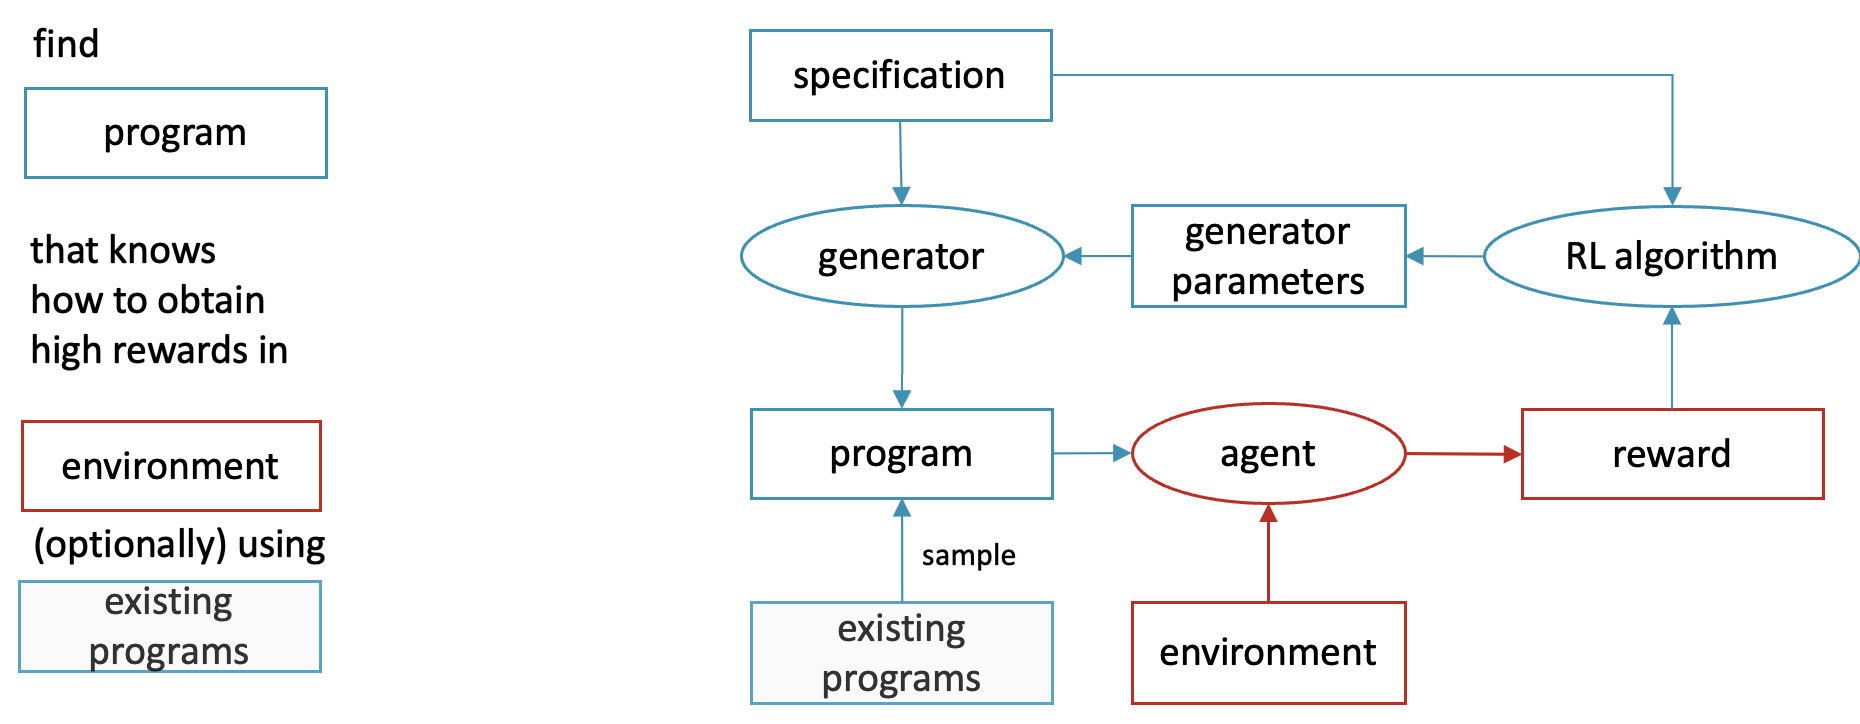
\includegraphics[width=\linewidth]{pirl.png}
    \caption{Reinforcement Learning From Code Execution Feedback, schematic definition}
    \label{fig:RLCEF}
\end{figure}

In this setting, each generated program is tested (see \textcolor{accent}{test} in figure \ref{fig:ap}) via deployment of an \textcolor{accent}{agent} controlled by this program in an environment that responds with positive and negative \textcolor{accent}{rewards} (the highlights of figure \ref{fig:RLCEF} match the highlights of this sentence).
The fitness of the program is then determined by the total reward collected by the agent during such a deployment (also known as an \emph{episode}).

The most common formalism for such an environment is Episodic Partially Observable Markov Decision Process \cite{kramerjdavidrPartiallyObservableMarkov1964, spaanPartiallyObservableMarkov2012}: when at step $i$ the agent takes action $a_i \in \actions$ it has an impact on  the state of the environment $s_i \in \states$ via distribution $\prob_\state(\state_{\step+1} | \step_\step, \action_\step)$ of conditional probabilities of possible subsequent states. 
State $\state$ is a latent variable that the agent cannot observe.
Instead, the agent has access to an observation $o_i \in \obss$ which is a random variable that depends on the latent state via distribution $\prob_\obs(\obs_\step | \state_\step, \action_\step)$.
$\actions$, $\states$ and $\obss$ are sets of all possible actions, states and observations respectively.
Finally, at every step the agent observes a reward $\reward(\state_\step,\action_\step)$.
The agent's goal is then to maximize its expected $n$-step return $\expectation [ \sum_{t=i}^{n} r_t ]$. Outside of explicitly stated special cases, the agent's planning horizon $n$ is always set equal to the length of the episode.

\newpage
\section{Why not just use Machine Learning?}
\label{sec:whynotml}

As programmatically interpretable cousins of \emph{supervised learning} and \emph{reinforcement learning} respectively, \emph{Programming by example} and \emph{RLCEF} are  used in settings where more traditional machine learning methods that do not involve code generation could also be used.
What are then the advantages conferred by this programmatic representation?

\subsection{Expressiveness and performance}
\begin{remark}
    A reproducibility package for this experiment has been published at \cite{Vadim0x60FizzbuzzlmSearching}
\end{remark}

Programming languages benefit from decades of research into making them \textcolor{accent}{expressive} - able to efficiently represent any algorithm one can design - and \textcolor{accent}{performant} - making those algorithms executable with minimal requirements of time and hardware.
Machine learning models do not have this advantage - they are designed to make the space of possible models easy to search and optimize in, often at the expense of expressivity and performance: on these criteria they can be so inadequate as to become a setup of programmer humor \cite{JoelGrusFizz}.

In fact, \cite{JoelGrusFizz} underestimates the inefficiency of the neural approach, since it only implements FizzBuzz \cite{reesFizzBuzz1012002} classification as a neural network, while their text output system remains symbolic.
We correct for this and train a specialized language model for FizzBuzz task, benchmarking it against equivalent programs in major programming languages.

\begin{table}[H]
    \centering
    \begin{tabular}{r|r|l}
         Language & source, bytes & CPU runtime \\
         \midrule
         C & 321 & 340.3 µs ± 117.0 µs \\
         Rust & 307 & 573.5 µs ± 114.3 µs \\
         Go & 295 & 966.5 µs ±  93.2 µs \\
         Haskell & 213 & 16.1 ms ± 0.4 ms \\
         Java & 403 & 28.9 ms ± 0.6 ms \\
         JavaScript & 162 & 30.1 ms ± 0.4 ms \\
         Python & 192 & 44.9 ms ± 0.6 ms \\
         C\# & 289 & 60.4 ms ± 4.8 ms \\
         Clojure & 178 & 507.2 ms ± 6.5 ms \\
         FizzBuzzLM & 13177 & 853.2 ms ± 6.8 ms
         %\footnote{GPU (NeuralEngine) accelerated runtime was even slower, at 1.596 s ± 0.037 s}
    \end{tabular}
    \caption{Performance charecteristics of different FizzBuzz implementations}
    \label{tab:my_label}
\end{table}

We can see that the programming language implementations are somewhat faster than \emph{FizzBuzzLM} and much more expressive with at least \emph{FizzBuzzLM} 2 orders of magnitude behind the true Kolmogorov complexity \cite{kolmogorov} of the problem.
The only reason these performance costs are accepted is that it's easier to implement optimization in the space of possible neural network parameters than in the space of possible programs. 
When the problem of optimal program synthesis is solved, it becomes the "best of both worlds" approach: data-driven and trainable, but using an expressive and performant representation.
 
\subsection{Import and export of knowledge}
\label{sec:importexport}

Programs as a representation for decision-making of a model have a chance to become the \emph{lingua franca} for representing decision processes as they can be understood by a wide variety of intelligent systems, including humans and machine learning models. 
This enables humans and robots attempting to tackle the same problem to learn from each other.

\begin{figure}
    \centering
    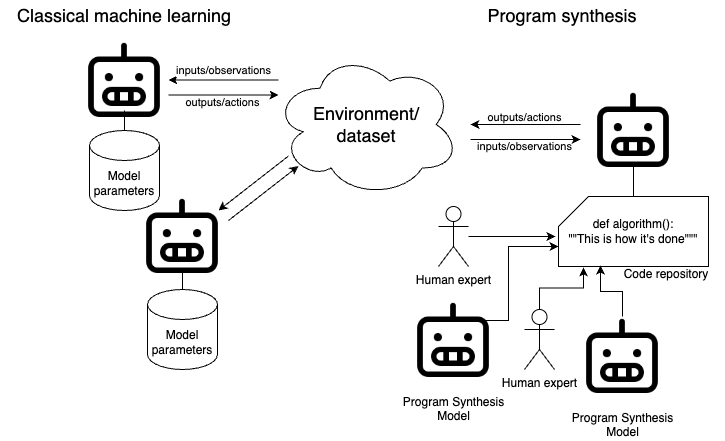
\includegraphics[width=\linewidth]{mlvsautocode.png}
    \caption{Program synthesis allows for knowledge sharing}
    \label{fig:mlvsautocode}
\end{figure}

The search in a space of possible programmatic solutions to a problem can be initialized with an existing program that has been developed by a subject area expert (perhaps with auxiliary use of automation), thus \textcolor{accent}{importing existing knowledge} from previous efforts of solving the same problem.
This process is not dissimilar to what is known in deep learning as \emph{fine-tuning}: initializing the optimization process of model parameters with a model already trained on a similar task, but it has the additional advantage that the initial code can be generated by a model of a completely different architecture or by a human.

After the search process has been concluded, all of the knowledge incorporated into the resulting system can be \textcolor{accent}{examined and verified}. 
Unlike the black-box model, the approach makes it trivial to answer questions like "Does this model include factor X in its decision-making on topic Y?".
This offers us an additional way of verifying the decision system before its final deployment. 
And, unlike the numerous post-hoc methods of machine learning interpretability \cite{linardatosExplainableAiReview2020}, this approach involves a strong guarantee by construction that the explanation does not diverge from the behavior.

Of course, external observers of a program synthesis system can act not only as teachers, but also as students. 
Even if the resulting program is never deployed, one can read it and \textcolor{accent}{export the knowledge} and incorporate it into future systems, as well as textbooks and other didactic materials for humans.

\newpage
\section{Broader impacts}
\label{sec:impacts}

\epigraph{The Future's So Bright, \\ I Gotta Wear Shades}{Timbuk 3}

\subsection{Capability}

The \emph{expressivity and performance} of programming languages can lead to \emph{decision support systems}, also known as \emph{digital assistants}, that are more capable, able to make more accurate predictions and provide better recommendations.

The ability to \emph{import, verify and export knowledge} into or out of a decision suport system can reduce or even eliminate \emph{knowledge silos} in the world, where each separate system has been trained on some data set of its own and some expert knowledge of its own and thus each incorporates some small part of all existing knowledge about the field. 

Insufficient capability in digital assistants is a major safety risk, especially when deployed fully autonomously. For example, misidentification of obstacles in autonomous driving \cite{sheebajoiceObstacleDetectionSafe2023} or wrongful diagnosis in healthcare \cite{wintersDiagnosticErrorsIntensive2012} can be a matter of life and death.

\subsection{Alignment}

Highly capable digital assistants present their own family of safety risks. 
If perverse incentives are present in the optimization goals of the decision system, then a highly capable decision system can bring about harmful situations intentionally.
Most optimization targets are imperfect proxies of intended outcomes. 
An optimization process can thus \emph{game} (\emph{hack}) the metrics and achieve negative outcomes, despite technically improving the metrics.
Common types of \emph{reward hacking} \cite{skalseDefiningCharacterizingReward2022} include:
\begin{description}
    \item[reward tampering] \cite{everittRewardTamperingProblems2021, skalseInvariancePolicyOptimisation2023} - acting on the reward mechanism directly, i.e. disabling sensors involved in the information chain that results in a negative reward or documenting once's actions with unwarranted optimism.
    \item[adverse selection] - selectively solving subtasks that are easier for the agent to solve even if they happen to be less important.
\end{description}

To give a real world example, both phenomenons have been observed in Healthcare: \cite{shenSelectionIncentivesPerformance2003} find that incentives can lead to the most severely ill patients being less likely to receive care. \cite{fairbrotherImpactFinancialIncentives2001, fairbrotherImpactPhysicianBonuses1999, roskiImpactFinancialIncentives2003} find that metrics are sometimes improved by better documenting the incentivized results, not improving them.
\cite{longFairnessMachineLearning2021} notes how misguided fairness metrics incentivize decision systems to intentionally harm people from healthier demographic groups in order to advance equality of outcomes ("equity").

These issues are present in society \cite{nestianPerverseIncentiveGeneral2017} with or without artificial intelligence, they are studied in economics under the umbrella of the \emph{principal agent problem} \cite{pandaAgencyTheoryReview2017}. 
However, powerful optimization algorithms have potential to exacerbate those issues \cite{hadfield-menellIncompleteContractingAI2019}. 
And while the first line of defense is, of course, improving the incentives, one can be skeptical as to whether the incentives can ever represent their designers' intentions perfectly.

In fact, the instrumental convergence theory \cite{benson-tilsenFormalizingConvergentInstrumental,bostromSuperintelligencePathsDangers2016} posits that perverse incentives are inherent to any reinforcement learning context, because optimizing for any goal can be aided by pursuing one of the basic drives \cite{omohundroBasicAIDrives2018}: self-preservation and improvement, rationality and accumulation of resources.
For example, a home climate control system can achieve its goals better the more devices in the user's house it controls: this creates an incentive to hack into heat-emitting appliances to be able to power them down on a hot day.
First introduced in science fiction \cite{clarke2001SpaceOdyssey2016, ellisonHaveNoMouth1967, jonesColossus2019}, this is now an active area of technical research \cite{jiAIAlignmentComprehensive2024}.
Estimates of the potential dangers of misaligned artificial intelligence range from non-trivial to existential \cite{mcleanRisksAssociatedArtificial2023}.

The interpretability afforded by the program synthesis approach provides a second line of defense against perverse incentives, namely, examining the control program and trying to establish whether any of the modules in that program are attempting to game the optimization metrics, manually or with the use of intelligent tools.

\begin{figure}
    \centering
    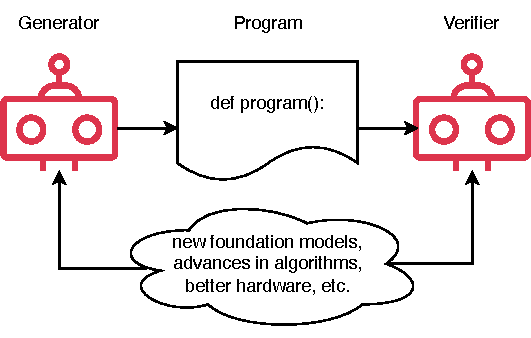
\includegraphics{PSAlign.drawio}
    \caption{Program Synthesis as an alignment methodology}
    \label{fig:ps-as-alignment}
\end{figure}

As technology advances, this advances both the generative tools and the verification tools, making program synthesis a promising approach to scalable oversight \cite[sec. 5]{amodeiConcreteProblemsAI2016}.

\subsection{Human-Robot Teams}

Transparency is a foremost principle of effective teamwork: every member of the team is supposed to know what and why every other member is doing. 
This principle is supported by the study of human teams \cite{bagPeerTransparencyTeams2012, solomonInferenceTransparencyEffective2021} and human-robot teams \cite{ezenyilimbaImpactTransparencyExplanations2022, guznovRobotTransparencyTeam2019, holderDesigningBiDirectionalTransparency2021, lakhmaniExploringEffectCommunication2019, lakhmaniProposedApproachDetermining2016, mercadoIntelligentAgentTransparency2016, ososkyDeterminantsSystemTransparency2014, panganibanTransparencyAutonomousTeammates2020, ronconeTransparentRoleAssignment2017} alike.
Some literature in Human-Robot teams takes inspiration \cite{shivelyCrewResourceManagement2018} from teamwork research in aviation where studies into the common causes of incidents and accidents \cite{chidesterPersonalityFactorsFlight1990, chidesterPilotPersonalityCrew1991, smithSimulatorStudyInteraction1979} have been used to formulate core principles of Crew Resource Management, such as "Verbalize Verify Monitor".
And as more automation is introduced in aviation, the modern cockpit itself can be seen as a human robot team.
Same is true of an operating theater with a robot assistant \cite{weerarathnaHumanRobotCollaborationHealthcare2023} or a doctor using a clinical decision support system \cite{castilloConsiderationsSuccessfulClinical2013, mooreIntroductionClinicalDecision2011, osullivanDecisionTimeClinical2014, purcellWhatMakesGood2005, sakallarisClinicalDecisionSupport2000, selfClinicalDecisionSupport2008, stangeThisIssueClinical2011, wrightClinicalDecisionSupport2009}

The lack of transparency is an important roadblock for integration of black box decision systems in safety critical domains: when conflict arises between the opinion of the expert and the opinion of the system, a black box system offers no additional information for the resolution of the conflict. 
A program, on the other hand, offers the experts a way to explicitly examine why a certain advice is given and use this information to take or not take the advice into account. 
Consequently, a black box system can only be used to completely replace a certain job - any setting where a collaboration is required between a human and decision system requires some degree of transparency that can be afforded by technology like program synthesis. 
This ensures synergistic decision-making where the analysis of every participant is taken into account of the final decision.

\subsection{Compliance}

Both individual organizations and regulatory authorities often impose requirements onto decision systems that are impossible to effectively enforce without transparency. 
An audit has to be able to establish whether the system violates discrimination law \cite{hochDiscriminationSakeFairness2024, schererApplyingOldRules2019}, accounting standards \cite{julischComplianceDesignBridging2011} or clinical norms \cite{flodgrenExternalInspectionCompliance}.
These requirements are a major impediment to deployment of machine learning in regulated safety-critical domains such as aviation \cite{torensGuidelinesRegulatoryFramework2021, vidotQualificationAvionicSoftware2024} and healthcare \cite{granlundRegulatoryCompliantMLOpsOravizio2021}.
A program, on the other hand, can be audited and proven to be compliant. 
Program synthesis can bring all the advantages of big data-driven systems into such fields without necessitating a regulatory reform.
These concerns become increasingly relevant as explainability of intelligent systems evolves from an implicit legal incentive \cite{hackerExplainableAIContract2020} to an explicit requirement \cite{linardatosExplainableAiReview2020}.

\subsection{Privacy}

The ineffiency of inference of current machine learning models is (along with competitive pressures) a core reason of the "cloudification" of machine learning: as of 2024, the most powerful models \cite{achiamGpt4TechnicalReport2023} are distributed as remote services that can be interacted with, but not fully copied, via the Internet.
Asking a state of the art decision support system for advice means sending the (potentially sensitive) request to the model provider and making both requests and responses known to said provider \cite{PrivacyPolicy}.
Programs, in contrast, are easier to distribute and performant enough to run on most devices most of the time.
The advent of program synthesis paves the way to more privacy-preserving decision support: even if the generative model remains in the cloud, one can first use the model to synthesize the program, then download it and submit the sensitive data to the program locally.

\subsection{Scientific discovery}

Lastly, export of knowledge out of a automatic programming system can be a powerful tool of scientific discovery. 
Symbolic regression is already widely used in physics in order to find formulas that fit experimental results \cite{angelisArtificialIntelligencePhysical2023, tenachiDeepSymbolicRegression2023}. 
In fact, it is not unreasonable to claim that physics \emph{is} a set of symbolic regression problems \cite{udrescuAIFeynmanPhysicsinspired2020}, historically solved manually, but increasingly with some application of algorithms. 
The same can be said about biology \cite{chenRevealingComplexEcological2019}, economics \cite{claveriaAssessmentEffectFinancial2017, lianModelingForecastingPassenger2018, panInfluentialFactorsCarbon2019, truscottDetectingShadowEconomy2011, truscottExplainingUnemploymentRates2014, yamashitaCustomizedPredictionAttendance2022} or any field that develops formulas based on series of empirical observations.
